\documentclass{standalone}
\usepackage{tikz}
\usepackage{amsmath}
\usetikzlibrary{3d}

\begin{document}
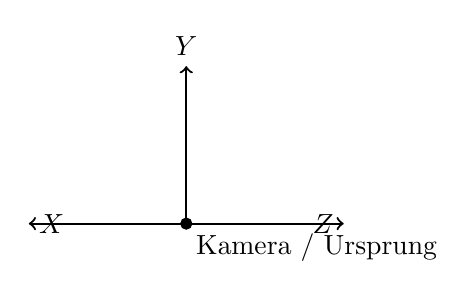
\begin{tikzpicture}[scale=2, x={(0cm,0cm)}, y={(0cm,1cm)}, z={(-1cm,0cm)}]

  % Ursprung
  \coordinate (O) at (0,0,0);

  % Achsen
  \draw[->, thick] (O) -- (0,1,0) node[above] {$Y$}; % Y: oben
  \draw[->, thick] (O) -- (0,0,-1) node[left] {$Z$}; % Z: nach links (optische Achse)
  \draw[->, thick] (O) -- (0,0.0,1) node[right] {$X$}; % X: heraus aus der Seite

  % Kameraursprung markieren
  \filldraw[black] (O) circle (1pt) node[below right] {Kamera / Ursprung};

\end{tikzpicture}
\end{document}